\section{Overview}

The baseline HBM2 device is organized as follows: 
base and core die slice which is stacked up to 8-Hi slices. 
The core die slice has 4 channels interconnected by TSV as shown Figure~\ref{fig:ch3:basearch}, 
Each of which has four quadrants with 16 banks/quadrant. 
Each quadrant, a channel is assigned 128 TSV I/Os in the TSV area across the core slice. 
Currently, we assume that our baseline HBM2 device consists of 4-Hi slices. 
So individual channel has 32 banks divided into upper and lower slice group.

We introduce two terminologies to the baseline HBM2 design: \textit{sectors} and activation bit vector. 
The \textit{sector} is a minimum activation granularity of row buffer. 
We divide row buffer into 8~\textit{sectors} from previous partial activation schemes from \mycite{yb17} and \mycite{Zhang14}.

\begin{figure}[th]
    \centering
        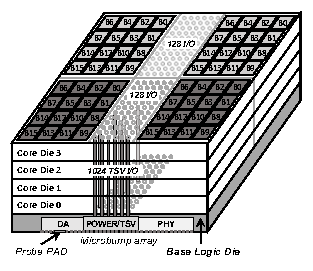
\includegraphics[page=1,width=0.5\linewidth]{figure/baseline_HBM2.pdf}
    \caption[Baseline HBM2 architecture]{Baseline HBM2 architecture\footnotemark{}}
    \label{fig:ch3:basearch}
\end{figure}

\section{Bank Structure}

\begin{figure}[th]
    \centering
        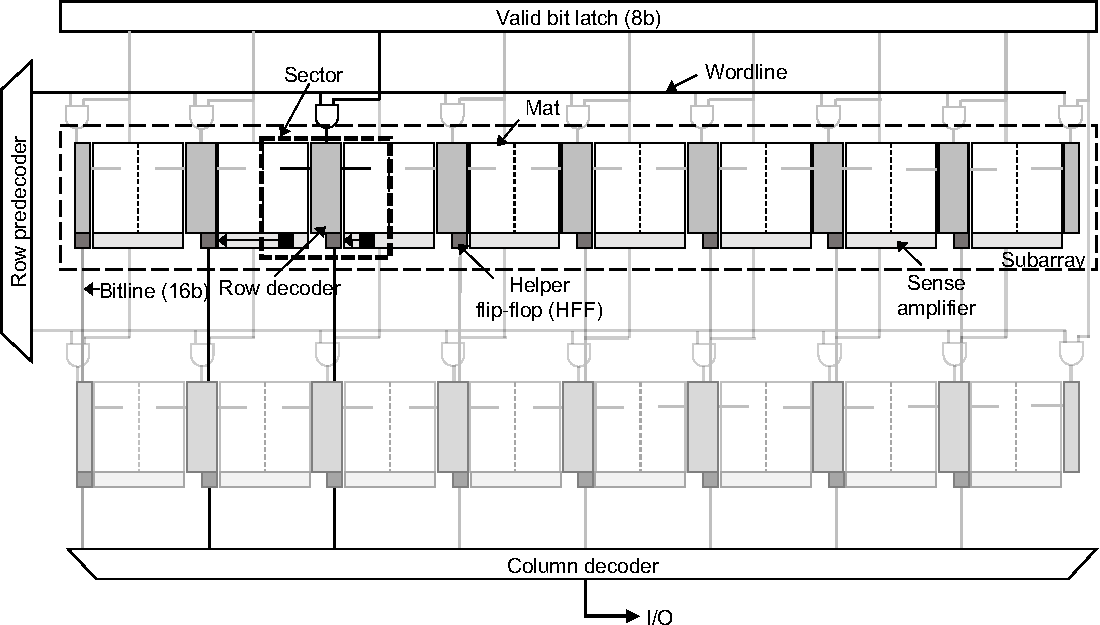
\includegraphics[width=\linewidth]{figure/bank_structure_vfin.pdf}
    \caption{Detailed view of PPA bank architecture}
    \label{fig:ch3:bankstruct}
\end{figure}

\footnotetext{Reproduced from \mycite{IMW17}} % HBM2 PKG fig citation
Figure~\ref{fig:ch3:bankstruct} 
shows the structure of a bank for our proposed DRAM architecture based on HBM2. A single bank consists of multiple subarrays, each of which is further divided into 8 mats sharing the same global word line. With the row size of 1KB, activating a single mat reads out 128B of row data, which is a common cacheline size for GPUs. Exploiting this characteristic, we re-organize the column address mapping of mats so that one mat houses a whole 32B column. To enable an activation of a single mat (instead of all eight), we simply add AND gates to the global word line. Such design increases the time to process a {\tt READ/WRITE} command by 14 memory cycles as it takes 14 extra cycles to burst out a 32B atom through a 16-bit-wide datapath (16 memory cycles in total) instead of a 128-bit-wide datapath (2 memory cycles in total).

To mitigate the effect on {\tt READ/WRITE} processing time from a narrower path to I/O, we also employ a proposal similar to half-DRAM~\mycite{Zhang14}. The main intuition of the Half-DRAM proposal is that it is possible to utilize two set of bitlines (and helper flip-flops (HFFs)) for activating a single DRAM cell worth of data by making a row decoder drives two half mats (the right half of the mat on the left and the left half of the mat on the right) instead of a single mat. As shown in Figure \ref{fig:ch3:bankstruct}, two half mats now utilize two sets of the 16 bitlines and this reduces the {\tt READ/WRITE} processing time to 8 memory cycles (i.e., 6-cycle increase). Note that we modify column mapping of mats so that a whole column address fits in two corresponding half mats. Throughout the paper, we call these two corresponding half mats a {\it sector} as shown in Figure~\ref{fig:ch3:bankstruct}.

To handle this increase in {\tt READ/WRITE} command processing time, we need to adjust DRAM's timing parameters. First, timing parameter {\tt tAA}, which represents the time between the read command and the first data output on bus, needs to be increased as the proposed bank structure requires extra cycles to output the data.  So {\tt tAA} is increased by 6 memory cycles. 
\begin{figure}[t]
    \centering
        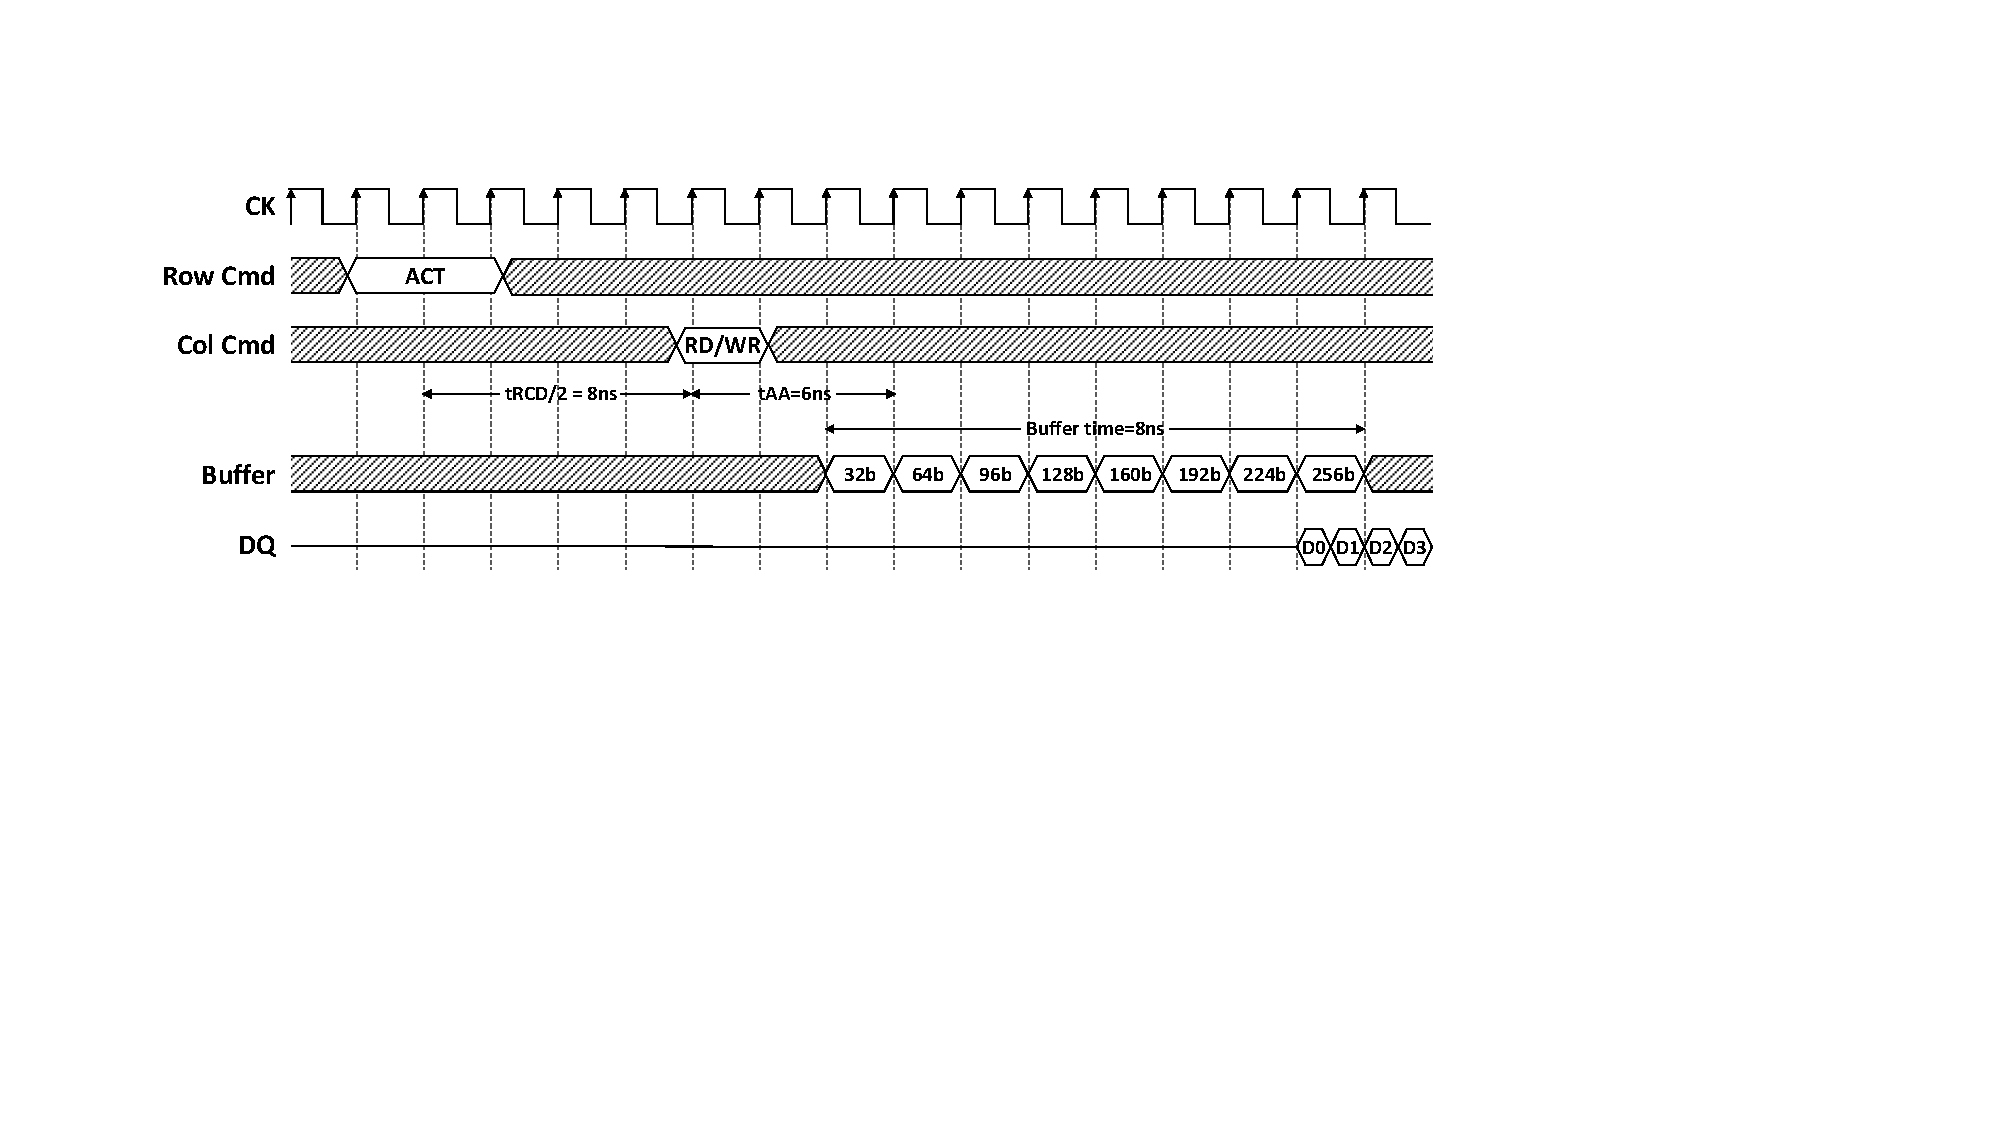
\includegraphics[width=\linewidth]{figure/data_fetch_time.pdf}
    \caption{Data fetch timing diagram through the narrow bitline}
    \label{fig:ch3:datfetch}
\end{figure}

Figure~\ref{fig:ch3:datfetch} above describes how the {\tt tAA} timing is lengthened 
when data being fetched by a cycle-by-cycle waveform. After corresponding {\it sector} activated, 
the 16-bit-wide bitlines on both sides are utilized to buffer the requested 32B data. 
The data is fetched 32 bits per cycle, and it takes 8 cycles to fetch 256 bits.
Since the first cycle of fetch data and {\tt tAA} timing can overlap, and the last fetch and two bursts 
can overlap, thus it takes a total of 6 cycles to buffer the data through the narrow bitline.

The timing between column commands to the same bank has to be increased. While a memory controller compliant to HBM standards already has {\tt tCCD}, column command to column command delay, we need a variation of this because we only need to increase the delay between column command to column command {\it to the same bank}. We denote this parameter {\tt tCCD}$_S$ and set it to {\tt tCCD}+6. This requires a slight timing change to the memory controller. Lastly, other {\tt READ/WRITE} related delays (e.g., {\tt tWR}, {\tt tWTR}, and {\tt tRTP}) needs to be increased by six cycles as well.

While these mechanisms reduce the peak bank bandwidth by up to 4$\times$ since the time it takes to handle a single {\tt READ/WRITE} command increases to 8 cycles from 2 cycles. However, this often does not lead to a decrease in overall memory bandwidth since HBM2 specification over-provisions DRAM banks. For example, the evaluated configuration includes 32 banks per channel, where each bank can provide up to 128 bits/cycle. On the other hand, each channel, despite having 32 banks, supply data at 256 bits/cycle. Assuming balanced distributions across 32 banks, each bank only needs to supply 8 bits/cycle to saturate the channel bandwidth. In other words, each bank achieving 1/16$\times$ of its peak throughput is enough to saturate the channel in this case. For this reason, although our proposed bank structure reduces the peak throughput of a single bank by 4$\times$, it is unlikely to affect the overall memory throughput, which is often first limited by channel throughput.

\begin{figure}[b]
    \centering
        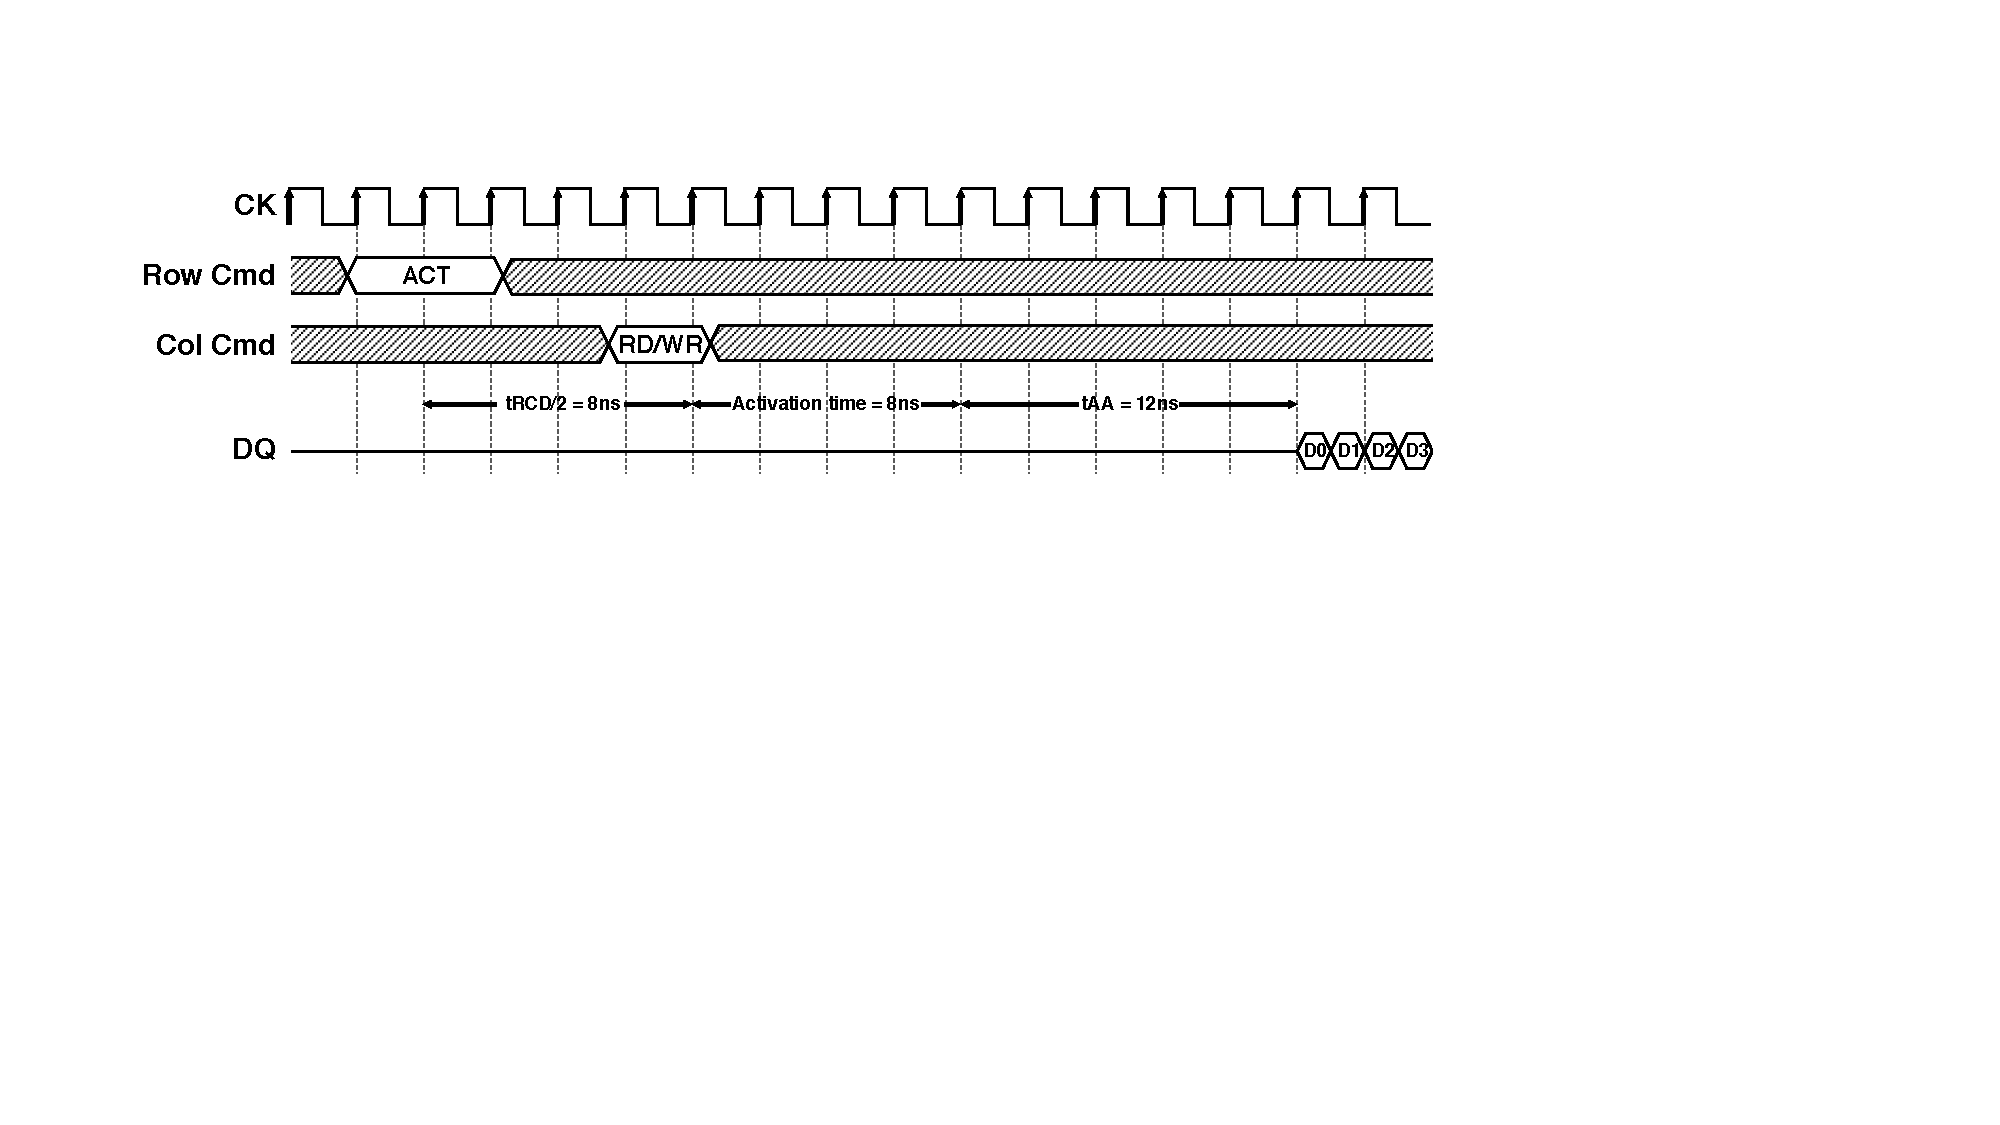
\includegraphics[width=\linewidth]{figure/waveform_del_act.pdf}
    \caption{Waveform of proposed delayed activation}
    \label{fig:ch3:delact}
\end{figure}

\section{Delayed Activation}
To specify which {\it sector} to activate we use delayed activation. When a DRAM device receives {\tt ACTIVATE} commands, the DRAM device decodes row address as usual but does not actually perform an activation and buffer the row address. Instead, the activation happens when a column command arrives. Once a column command (i.e., {\tt READ/WRITE}) arrives, the column address is first decoded and it is used to determine which DRAM {\it sector} it should activate. Then, a partial activation for that particular {\it sector} is performed and followed by actual READ/WRITE operation. Figure \ref{fig:ch3:delact} shows how this delayed activation scheme affects DRAM timing. First, since {\tt ACTIVATE} does not actually perform an activation, {\tt tRCD} becomes shorter (by half according to our estimation using CACTI-3DD \mycite{cacti3dd}). At the same time, since the activation happens in column commands, {\tt tAA} (i.e., the timing of read command to the first output data on the bus) and {\tt tWL} (i.e., the timing of write command to the first input data on the bus) should be increased by the reduced {\tt tRCD} amount. In our configuration, {\tt tRCD} is originally set to 16ns and thus {\tt tRCD} is reduced by 8ns while {\tt tAA} and {\tt tWL} are increased by 8ns. This scheme basically avoids unnecessary activation at the expense of potential 8ns extra latency for {\tt READ} and {\tt WRITE} command. The rationale behind this scheme is that such a minor increase in DRAM latency does not usually affect the performance of the latency-tolerant GPU workloads.

%The main idea of delayed activation is that we can only activate the exact amount of data we need in an on-demand basis. 
%According to the FR-FCFS policy, column accesses to the open row are prioritized over those to other rows.
%When a DRAM receives ACTIVATE commands, the DRAM device decodes row address as usual but does not actually perform an activation and buffer the row address. 
%Instead, the activation happens when a column command arrives. 
%Once a column command (i.e., {\tt READ/WRITE}) arrives, the column address is first decoded, and it is used to determine which DRAM \textit{sector} it should activate. 
%Then, a partial activation for that particular \textit{sector} is performed and followed by actual {\tt READ/WRITE} operation.
%When a DRAM request is headed to another row, a precharge must be performed first 
%as if a normal row buffer conflict occurred.
%
%Figure~\ref{fig:ch3:delact} shows how this delayed activation scheme affects DRAM timing. 
%First, since ACTIVATE does not actually perform an activation, $t_{RCD}$ becomes shorter 
%(half according to our estimation using CACTI-3DD~\mycite{cacti3dd}). At the same time, since the
%activation happens in column commands, $t_{AA}$ (i.e., the timing of read command to the first output 
%data on the bus) and $t_{WL}$ (i.e., the timing of write command to the first input data on the bus)
%should be increased by the reduced $t_{RCD}$ amount. 
%In our configuration, $t_{RCD}$ is originally set to 16ns and thus $t_{RCD}$ is reduced by 8ns while $t_{AA}$ and $t_{WL}$ are increased by 8ns. 
%This scheme basically trades-off an ability to avoid unnecessary activation at the expense of potential
%8ns extra latency for {\tt READ} and {\tt WRITE} command. 
%The rationale behind this scheme is that such a minor increase in DRAM latency does not usually affect the performance of latency-tolerant GPU workloads.
